\chapter{Testing, Results and Evaluation}
The following chapter will cover the steps taken for evaluating the model in terms of performance and accuracy. Several performance measures are used for determining how well the model handles data that it has not been trained with. These include training evaluation, testing with the testing data and inference with new data. Also, usability testing of the web application will be discussed in detail.

\section{Training Results and Evaluation}
During the training of the model, a number of metrics were recorded for evaluation its performance.  As mentioned in the machine learning model section of Chapter 3, The loss (often referred to as the cost function) is calculated by measuring the error of the predicted label in comparison to the true label. This is useful for determining the level of optimization being carried out on the network when using back propagation to adjust the weights. The closer the loss is to zero, the more accurate the model is at classifying. As seen in Figure \ref{loss}, the initially loss for the first epoch was approximately 185. This value decreased gradually throughout the training of the network, getting closer to 0.

\begin{figure}[ht]
	\begin{center}
		\advance\leftskip-3cm
		\advance\rightskip-3cm
		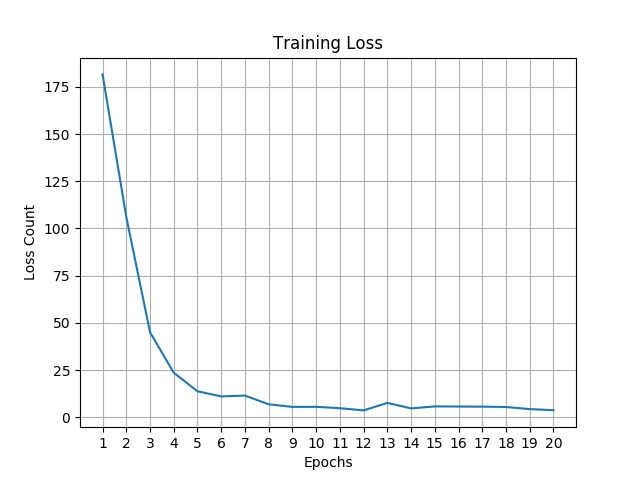
\includegraphics[keepaspectratio=true,scale=0.7]{__resources/Results/loss.jpg}
		\caption{Loss Function Values}
		\label{loss}
	\end{center}
\end{figure}

\newpage

The second training measurement taken into account was the accuracy throughout each step in training. This is measure by the adding the true positive with the true negative results, and dividing the sum by the total number of samples in the dataset(See equation 6.1.1).


\begin{equation}\label{eq:ac}
Accuracy = 
\frac{
	True\ positive\ + Σ\ True\ negative
}{
	Total\ population
}
\end{equation}
Intuitively, it is desired to have the highest accuracy possible, but this may not always be the case, due to what is known as the accuracy paradox in predictive analytics. It is said that using accuracy is not a desirable method of measuring performance, as it can give misleading results if there is a high class imbalance, but this is not problem in our case as it was made certain that each class was represented equally in the preprocessing steps.  The level of accuracy throughout training was measured and plotted in graph for evaluation. See Figure \ref{acc}.

\begin{figure}[ht]
	\begin{center}
		\advance\leftskip-3cm
		\advance\rightskip-3cm
		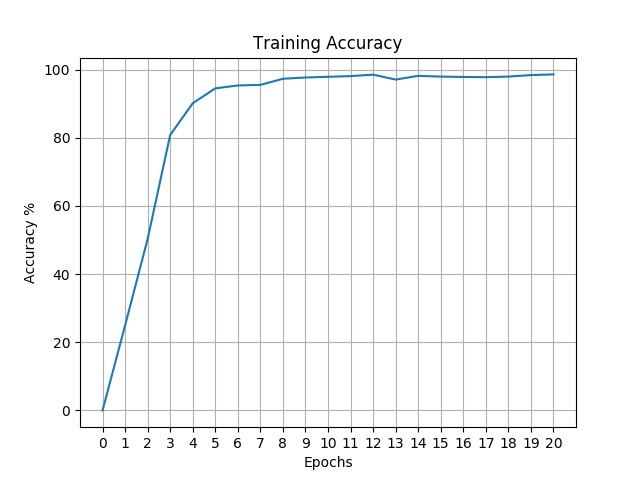
\includegraphics[keepaspectratio=true,scale=0.7]{__resources/Results/accuracy.jpg}
		\caption{Accuracy Values}
		\label{acc}
	\end{center}
\end{figure}

\newpage

\section{Testing Model with Testing Data}
As stated in the implementation chapter, the dataset was split into training and testing sets. out of the 1750 images for each class, 1400 of them were used for training, and the remaining 350 were used for testing the model's performance. A python evaluation script was used for loading each set of classes individually and feed them to the trained model. 

\begin{figure}[ht]
	\begin{center}
		\advance\leftskip-3cm
		\advance\rightskip-3cm
		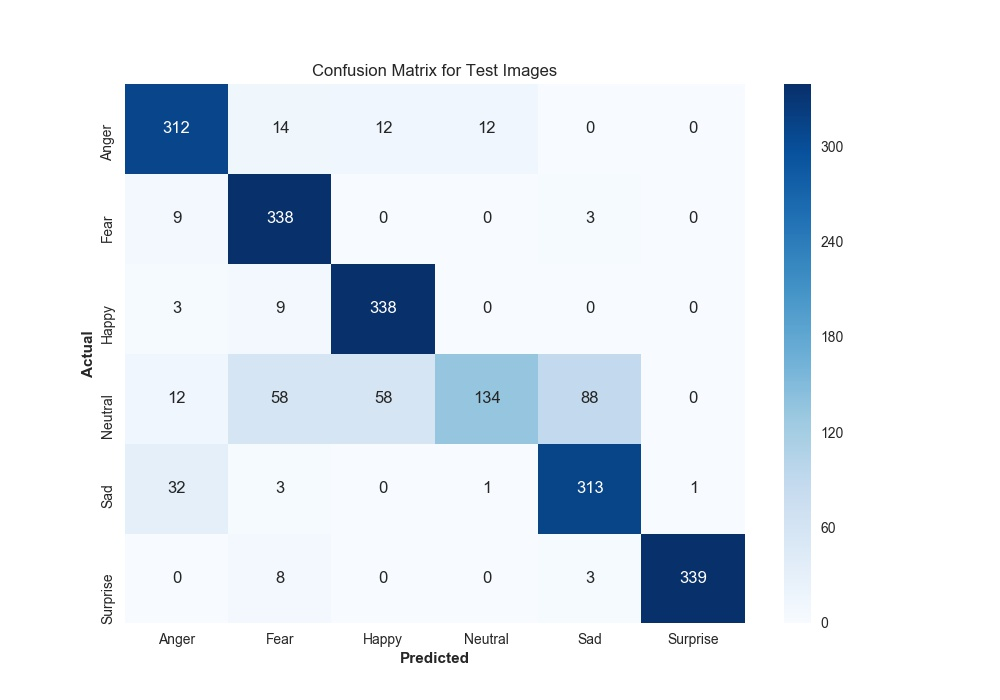
\includegraphics[keepaspectratio=true,scale=0.5]{__resources/Results/confusion.jpg}
		\caption{Confusion Matrix Heatmap}
		\label{conf}
	\end{center}
\end{figure}
\newpage

From this confusion matrix we are able to plot out a number of performance metrics besides the basic training accuracy and loss. Firstly, the recall of each is measured. The recall of a class can be described are the number of true positives divided by the number of true positives and false negatives, as seen in equation 6.2.1. 

\begin{equation}\label{eq:recall}
Recall = 
\frac{
True\ positive
}{
True\ Positive + False\ Negative
}
\end{equation}

Also, the precision of model can be calculated. The precision is a measure of the number of true positives classified divided by the sum of true positives and false positives, which can be seen in equation 6.2.2

\begin{equation}\label{eq:precision}
Precision = 
\frac{
	True\ positive
}{
	True\ Positive + False\ Positive
}
\end{equation}

From these equations the scores for recall, precision and accuracy are calculated using the data shown in Figure \ref{conf}. Also, the averages for each metric was calculated, as can be seen in Table \ref{table:per}.
\begin{table}[ht]
	\begin{center}
	\begin{tabular}{|p{5cm}||p{2cm}||p{2cm}|}		
		\hline
		
		\multicolumn{3}{|c|}{Testing Performance Measures} \\
		\hline
		\textbf{Class}& \textbf{Precision} &  \textbf{Recall}\\
		\hline
		Anger  & 84.7\% & 89.14\%	\\
		\hline
		Fear  & 78.6\% & 96.5\%	\\
		\hline
		Happy  & 82.8\% & 96.5\%  \\
		\hline
		Neutral & 91.15\% & 38.2\%	\\
		\hline	
		Sadness &  76.9\% & 89.4\%	\\
		\hline
		Surprise & 99.7 \% & 96.8\%	\\
		\hline	
		\hline 
		\textit{Accuracy} & \multicolumn{2}{|c|}{ 84.47\%} \\
		\hline
		\textit{Average Precision} & \multicolumn{2}{|c|}{ 85.64\%} \\
		\hline
		\textit{Average Recall} & \multicolumn{2}{|c|}{ 84.42\%} \\
		\hline
	\end{tabular}
	\caption{Table of Performance Measure Results}
	\label{table:per}
	\end{center}
\end{table}
	
\section{Testing Model with Single Inference}
Single inference was performed with images taken from Google Images to see how well the model performed without any of the preprocessing steps. One image was chosen at random for each emotion. See Figure \ref{inf}.

\begin{figure}[ht]
	\begin{center}
		\advance\leftskip-3cm
		\advance\rightskip-3cm
		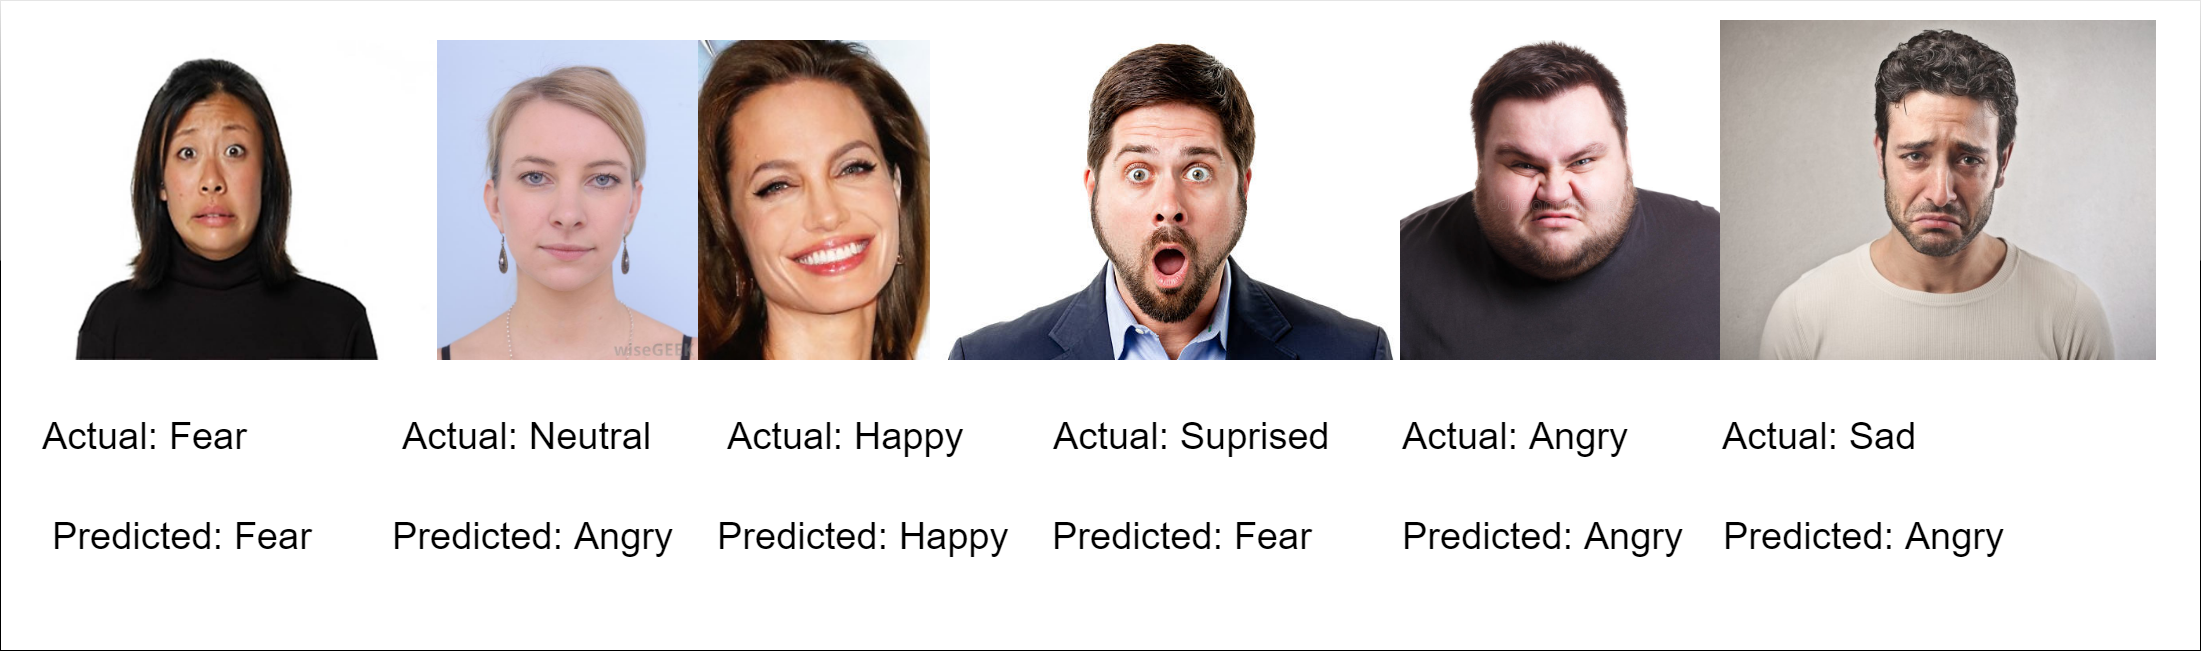
\includegraphics[keepaspectratio=true,scale=0.21]{__resources/Testing/inference.png}
		\caption{Single Predictions on Non-preprocessed Images}
		\label{inf}
	\end{center}
\end{figure}


\section{Usability Testing}
After model was deployed to the web application, some black box testing was performed. For each of the emotion classes, a 30-snapshot test was conducted using the same facial expression to determine how well the model would classify using the data from the web application. The same facial expression was trailed three times each and the average scores were recorded. These results are percentages of how many times the model classified a certain emotion. Results are shown in Table \ref{table:use}


\begin{table}[ht]
	\begin{center}
		\begin{tabular}{|c|c|c|c|c|c|c|}		
			\hline 
			Predicted & \textbf{Anger} &  \textbf{Fear} & \textbf{Happiness} & \textbf{Neutral} & \textbf{Sadness}& \textbf{Surprise}\\
			\hline 
			Anger & \textbf{71\%} &0\% &8\% & 43\%& 59\% & 17\%\\
			\hline 
			Fear & 29\% & \textbf{89\%} & 0\%& 32\%&0\% & 57\%\\
			\hline 
			Happiness &0\% &11\% &\textbf{92\%} & 11\%&0\% &23\% \\
			\hline 
			Neutral & 0\% &0\% &0\% & \textbf{0\%}&0\% &0\% \\
			\hline 
			Sadness & 0\%&0\% &0\% & 3\%& \textbf{41\% }&1\% \\
			\hline 
			Surprise & 0\%&0\% &0\% & 11\%&0\% & \textbf{2\%}\\
			\hline
		\end{tabular}
		\caption{Usability Testing Results}
		\label{table:use}
	\end{center}
\end{table}
\newpage


\section{Concluding Remarks of Testing and Evaluation}
In conclusion, the training performance evaluation was discussed in regard to the loss and accuracy of the model during the training stage.
The loss begins at approximately 185 and is deduced to 3.0 upon the completion of training. The final accuracy displayed in Figure \ref{acc} displayed a high score of approximately 98\%.

Testing was done on the trained mode l with 350 images per class with a highly correct classification score excluding the neutral class. Recall and precision scores were calculated using a confusion matrix. The neutral class did not have as high of an accurate classification score as the rest of the classes. A speculated reason for this might be because the facial features of the subject may just naturally appear like other facial features, such as sadness, which was classified 88 times out of 350. Also, it is possible that by the augmented images for this class may have morphed the image too much, therefore making them appear to look like another class (happy or sad in this case).

Inference was performed using randomly selected images sourced from Google images in order to examine how the model performed. In terms predictive performance the classifications were only moderately accurate (classifying 3/6 images correctly), but it should be noted that facial cropping needs to be performed on each image for more accurate results.

Lastly, the usability of the web application in conjunction with the trained and deployed model performed pretty good for some classes. Emotions such as happiness, anger and fear were very well classified when testing, as can be seen in Table \ref{table:use} . The other three classes however did not have as high as a classification percentage. The worst of which was the neutral class which was classified 0\% of the time during testing, which is evidently correlated with the fact that the model could not extract accurate features for the neutral class while training. Other factors should also be taken into account: Lighting, webcam quality and facial accessories such as glasses may have an affect and skew the results returned from the model as the dataset did not have the sufficient image data to deal with these conditions.



